\section{Risultati preliminari}
\subsection{Validazione del primo stadio di recupero}
Alla fine della prima epoca, dopo 450 minibatch, la perdita media è 0,9766 (deviazione standard tra minibatch 0,6671). La frazione di positivi al primo posto tra i candidati di addestramento è 0,6328. Il tempo registrato per l'epoca è 3\,583 secondi. Valutare il ranking sull'intero corpus richiede il calcolo degli embedding di ciascuna collezione: per Earth Science, ad esempio, trascorrono circa 129 minuti dall'avvio della validazione di dominio alla disponibilità dei 121\,249 vettori. Il tempo dell'epoca da solo sottostima quindi il costo dell'esperimento.

La Tabella~\ref{tab:domains} riporta tutti i domini per i quali il log del 25 novembre documenta il completamento. Per Sustainable Living il log termina durante la codifica dei documenti; i suoi 32 turni restano fuori dal denominatore. Per ogni dominio calcoliamo la media di nDCG@10 sui turni; l'ultima riga assegna uguale peso ai dieci domini osservati. I valori derivano dai punteggi di dominio arrotondati a quattro decimali.
\begin{table}[htbp]\centering\small
\caption{nDCG@10 di validazione interna nell'epoca 1 del 2a. C indica la query contestuale, S la riscrittura. La fusione mista usa il denso S e BM25 C. I due gruppi di domini corrispondono a BRIGHT e StackExchange.}\label{tab:domains}
\setlength{\tabcolsep}{3pt}
\begin{tabular}{lr rr rr rrr}\toprule
& & \multicolumn{2}{c}{Denso} & \multicolumn{2}{c}{BM25} & \multicolumn{3}{c}{RRF}\\
\cmidrule(lr){3-4}\cmidrule(lr){5-6}\cmidrule(lr){7-9}
Dominio & Turni & C & S & C & S & C & S & Mista\\\midrule
Biology & 33 & 0.0689 & 0.0598 & 0.5649 & 0.4264 & 0.5329 & 0.4390 & 0.5142 \\
Earth Science & 46 & 0.1905 & 0.1702 & 0.6465 & 0.5940 & 0.6021 & 0.5363 & 0.6179 \\
Economics & 28 & 0.0376 & 0.0421 & 0.4041 & 0.4418 & 0.3279 & 0.3162 & 0.3171 \\
Psychology & 43 & 0.1792 & 0.1166 & 0.7077 & 0.5493 & 0.6701 & 0.5343 & 0.6497 \\
Robotics & 26 & 0.0904 & 0.0389 & 0.3652 & 0.3174 & 0.5197 & 0.4034 & 0.4665 \\
\midrule
Drones & 17 & 0.6197 & 0.6186 & 0.3342 & 0.3072 & 0.7473 & 0.6999 & 0.7582 \\
Hardware & 22 & 0.3229 & 0.3385 & 0.2377 & 0.1705 & 0.5987 & 0.5674 & 0.6234 \\
Law & 25 & 0.7169 & 0.7146 & 0.2818 & 0.1668 & 0.6890 & 0.5439 & 0.6902 \\
Medical Sciences & 21 & 0.7196 & 0.5936 & 0.1892 & 0.1310 & 0.7188 & 0.5070 & 0.6888 \\
Politics & 19 & 0.8555 & 0.7638 & 0.4361 & 0.3561 & 0.8352 & 0.7877 & 0.7885 \\
\midrule
Media macro & 280 & 0.3801 & 0.3457 & 0.4167 & 0.3461 & 0.6242 & 0.5335 & 0.6114 \\\bottomrule\end{tabular}\end{table}

La fusione contestuale raggiunge 0,6242 contro 0,4167 per BM25 e 0,3801 per il denso. La differenza rispetto a BM25 è particolarmente ampia in Drones (0,7473 contro 0,3342). In Biology, invece, BM25 supera la fusione (0,5649 contro 0,5329). Anche quando il denso individua un documento pertinente nella lista estesa, può collocarlo troppo in basso: in Biology il suo Recall@1000 è 0,9343, mentre il Recall@10 scende a 0,1439. Per i candidati di un riordinatore con $K=100$ il valore pertinente è Recall@100, qui pari a 0,5985 per il denso e 0,8434 per BM25.
\begin{figure}[htbp]\centering
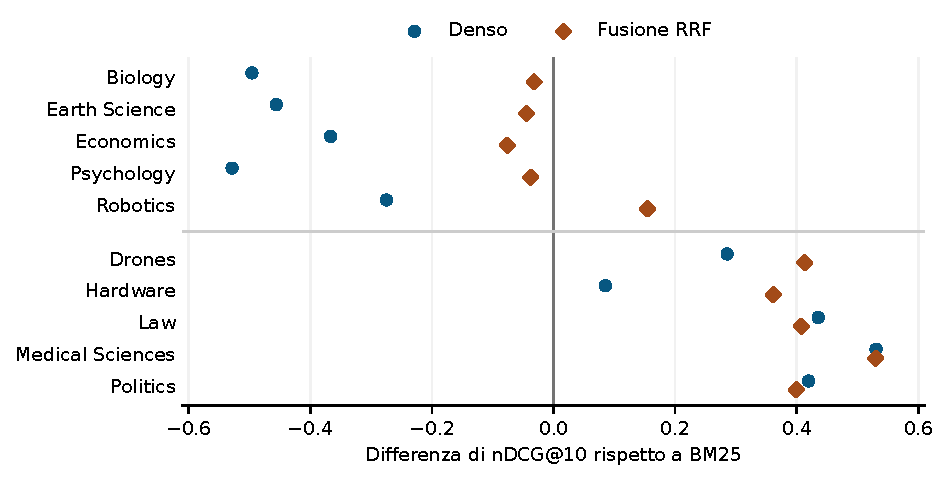
\includegraphics[width=.87\linewidth]{confronto_per_dominio.pdf}
\caption{Differenze rispetto a BM25 con la stessa query contestuale. A destra dello zero il sistema supera BM25. La linea orizzontale separa le due origini delle collezioni. Ogni punto è una differenza tra medie sullo stesso insieme di turni.}\label{fig:domains}
\end{figure}

\subsection{Misure previste per il confronto di profondità}
Per il 2a il confronto primario sarà $R=2$ contro $R=1$ sugli stessi candidati; $R=4$ servirà come analisi esplorativa di sensibilità. Per un dominio $d$, indichiamo con $m_{t,R}$ la nDCG@10 del turno $t$ alla profondità $R$. L'effetto principale sul dev sarà
\[
 \Delta_{2a}=\frac1{11}\sum_{d=1}^{11}\frac1{n_d}\sum_{t\in d}
 (m_{t,2}-m_{t,1}).
\]
Registreremo la copertura dei candidati prima del riordinamento, la latenza per query senza riuso dei punteggi e la memoria GPU di picco. Per quantificare l'incertezza prevediamo un bootstrap appaiato stratificato per dominio, ricampionando intere conversazioni e mantenendo insieme i loro turni. Gli intervalli al 95\% descriveranno la variabilità campionaria a checkpoint fissato.

Nel 2b il criterio primario proposto è la fedeltà ai passaggi; correttezza, completezza, pertinenza e coerenza conversazionale completano il profilo. Adotteremo la scala intera 1--5 per ciascuna dimensione e la trasformazione $(s-1)/4$ del protocollo RETECO \cite{evaluation}. Per una valutazione locale cieca, le risposte saranno anonimizzate e presentate in ordine casuale con domanda, storia ed evidenze identiche; conserveremo anche casi di parità e risposte mancanti. Prevediamo un secondo giudizio indipendente su un sottoinsieme per verificare l'accordo. Riporteremo le differenze appaiate, i token prodotti e i secondi per risposta. I log disponibili documentano il primo stadio del 2a; nessuna misura comparativa di profondità o di qualità delle risposte 2b è ancora disponibile.
